% 2005 年江西卷理科第 22 题：抛物线切线与焦点角
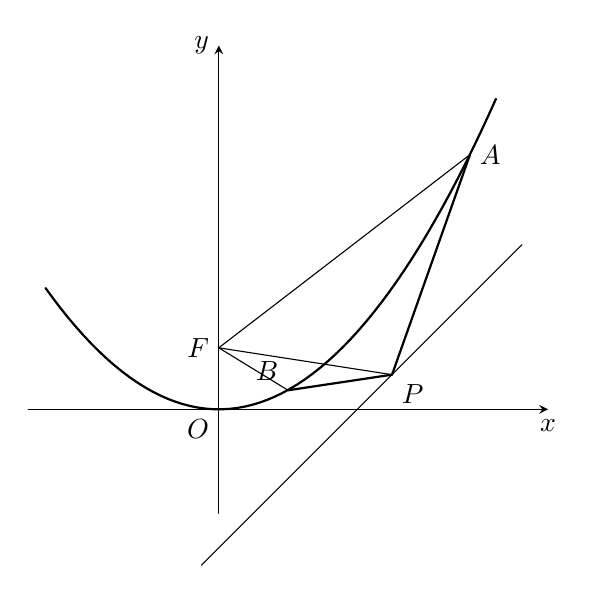
\begin{tikzpicture}[>=stealth,scale=1.1,line cap=round]
  % 坐标轴
  \draw[->] (-2.2,0) -- (3.8,0) node[below] {$x$};
  \draw[->] (0,-1.2) -- (0,4.2) node[left] {$y$};
  \node[below left] at (0,0) {$O$};

  % 抛物线 y = 0.35 x^2
  \draw[thick,domain=-2.0:3.2,samples=60] plot (\x,{0.35*\x*\x});

  % 关键点坐标
  \coordinate (F) at (0, 0.71);
  \coordinate (P) at (2.0, 0.4);
  \coordinate (A) at (2.9, 2.94);
  \coordinate (B) at (0.8, 0.22);

  % 直线 l: y = x - 1.6 通过 P(2.0, 0.4)
  \draw[domain=-0.2:3.5,samples=2] plot (\x,{\x - 1.6});

  % 切线 PA, PB
  \draw[thick] (P) -- (A);
  \draw[thick] (P) -- (B);

  % 焦点连线 FA, FB, FP
  \draw (F) -- (A);
  \draw (F) -- (B);
  \draw (F) -- (P);

  % 点标注
  \node[left] at (F) {$F$};
  \node[right] at (A) {$A$};
  \node[below right] at (P) {$P$};
  \node[above left] at (B) {$B$};
\end{tikzpicture}
